
%{{第四十五回}}{第四十五回}}

\chapter{金兰契互剖金兰语\hspace{.5em}风雨夕闷制风雨词}

{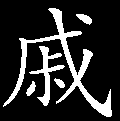
\includegraphics[width=3mm]{../Images/00005}  \kaishu 富贵荣华春暖,梦破黄{{(粮)}}{[}粱{]}愁晚。金玉作楼台,也是戏场妆点。莫缓,莫缓,遗却灵光不远。}

话说凤姐儿正抚恤平儿,忽见众姊妹进来,忙让坐了,平儿斟上茶来。凤姐儿笑道:``今儿来的这么齐,倒像下帖子请了来的。''探春笑道:``我们有两件事:一件是我的,一件是四妹妹的,还夹着老太太的话。''凤姐儿笑道:``有什么事,这么要紧?''探春笑道:``我们起了个诗社,头一社就不齐全,众人脸软,所以就乱了。我想必得你去作个监社御史,铁面无私才好。再四妹妹为画园子,用的东西这般那般不全,回了老太太,老太太说:`只怕后头楼底下还有当年剩下的,找一找,若有呢拿出来,若没有,叫人买去。'''凤姐笑道:``我又不会作什么湿的干的,要我吃东西去不成?''探春道:``你虽不会作,也不要你作。你只监察着我们里头有偷安怠惰的,该怎么样罚他就是了。''凤姐儿笑道:``你们别哄我,我猜着了,那里是请我作监社御史!分明是叫我作个进钱的铜商。你们弄什么社,必是要轮流作东道的。你们的月钱不够花了,想出这个法子来拗了我去,好和我要钱。可是这个主意?''一席话说的众人都笑起来了。李纨笑道:``真真你是个水晶心肝玻璃人。''凤姐儿笑道:``亏你是个大嫂子呢!把姑娘们原交给你带着念书学规矩针线的,他们不好,你要劝。这会子他们起诗社,能用几个钱,你就不管了?老太太、太太罢了,原是老封君。你一个月十两银子的月钱,比我们多两倍银子。老太太、太太还说你寡妇失业的,可怜,不够用,又有个小子,足的又添了十两,和老太太、太太平等。又给你园子地,各人取租子。年终分年例,你又是上上分儿。你娘儿们,主子奴才共总没十个人,吃的穿的仍旧是官中的。一年通共算起来,也有四五百银子。这会子你就每年拿出一二百两银子来陪他们顽顽,能几年的限?他们各人出了阁,难道还要你赔不成?这会子你怕花钱,调唆他们来闹我,我乐得去吃一个河涸海干,我还通不知道呢!''

李纨笑道:``你们听听,我说了一句,他就疯了,说了两车的无赖泥腿市俗专会打细算盘、分斤拨两的话出来。{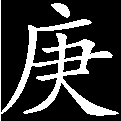
\includegraphics[width=3mm]{../Images/00004}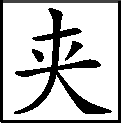
\includegraphics[width=3mm]{../Images/00012}\footnotesize \kaishu 心直口拙之人急了,恨不得将万句话来并成一句,说死那人,毕肖!}这东西亏他托生在诗书大宦名门之家做小姐,出了嫁又是这样,他还是这么着;若是生在贫寒小户人家,作个小子,还不知怎么下作贫嘴恶舌的呢!天下人都被你算计了去!昨儿还打平儿呢,亏你伸的出手来!那黄汤难道灌丧了狗肚子里去了?气的我只要给平儿打抱不平儿。忖夺了半日,好容易`狗长尾巴尖儿'的好日子,又怕老太太心里不受用,因此没来,究竟气还未平。你今儿又招我来了。给平儿拾鞋也不要,你们两个只该换一个过子才是。''说的众人都笑了。凤姐儿忙笑道:``竟不是为诗为画来找我,这脸子竟是为平儿来报仇的。竟不承望平儿有你这一位仗腰子的人。早知道,便有鬼拉着我的手打他,我也不打了。平姑娘,过来!我当着大奶奶姑娘们替你赔个不是,担待我酒后无德罢。''说着,众人又都笑起来了。李纨笑问平儿道:``如何?我说必定要给你争争气才罢。''平儿笑道:``虽如此,奶奶们取笑,我禁不起。''李纨道:``什么禁不起,有我呢。快拿了钥匙,叫你主子开了楼房找东西去。''

凤姐儿笑道:``好嫂子,你且同他们回园子里去。才要把这米账合算一算,那边大太太又打发人来叫,又不知有什么话说,须得过去走一趟。还有年下你们添补的衣服,还没打点给他们做去。''李纨笑道:``这些事情我都不管,你只把我的事完了我好歇着去,省得这些姑娘小姐闹我。''凤姐忙笑道:``好嫂子,赏我一点空儿。你是最疼我的,怎么今儿为平儿就不疼我了?往常你还劝我说,事情虽多,也该保养身子,捡点着偷空儿歇歇,你今儿反倒逼我的命了。况且误了别人的年下衣裳无碍,他姊妹们的若误了,却是你的责任,老太太岂不怪你不管闲事,这一句现成的话也不说?我宁可自己落不是,岂敢带累你呢。''李纨笑道:``你们听听,说的好不好?把他会说话的!我且问你:这诗社你到底管不管?''凤姐儿笑道:``这是什么话,我不入社花几个钱,不成了大观园的反叛了,还想在这里吃饭不成?明儿一早就到任,下马拜了印,先放下五十两银子给你们慢慢作会社东道。过后几天,我又不作诗作文,只不过是个俗人罢了。`监察'也罢,不`监察'也罢,有了钱了,你们还撵出我来!''说的众人又都笑起来。凤姐儿道:``过会子我开了楼房,凡有这些东西都叫人搬出来你们看,若使得,留着使,若少什么,照你们单子,我叫人替你们买去就是了。画绢我就裁出来。那图样没有在太太跟前,还在那边珍大爷那里呢。说给你们,别碰钉子去。我打发人取了来,一并叫人连绢交给相公们矾去。如何?''李纨点首笑道:``这难为你,果然这样还罢了。既如此,咱们家去罢,等着他不送了去再来闹他。''说着,便带了他姊妹就走。凤姐儿道:``这些事再没两个人,都是宝玉生出来的。''李纨听了,忙回身笑道:``正是为宝玉来,反忘了他。头一社是他误了。我们脸软,你说该怎么罚他?''凤姐想了一想,说道:``没有别的法子,只叫他把你们各人屋子里的地罚他扫一遍才好。''众人都笑道:``这话不差。''

说着才要回去,只见一个小丫头扶了赖嬷嬷进来。凤姐儿等忙站起来,笑道:``大娘坐。''又都向他道喜。赖嬷嬷向炕沿上坐了,笑道:``我也喜,主子们也喜。若不是主子们的恩典,我们这喜从何来?昨儿奶奶又打发彩哥儿赏东西,我孙子在门上朝上磕了头了。''李纨笑道:``多早晚上任去?''赖嬷嬷叹道:``我那里管他们,由他们去罢!前儿在家里给我磕头,我没好话,我说:`哥哥儿,你别说你是官儿了,横行霸道的!你今年活了三十岁,虽然是人家的奴才,一落娘胎胞,主子恩典,放你出来,上托着主子的洪福,下托着你老子娘,也是公子哥儿似的读书认字,也是丫头、老婆、奶子捧凤凰似的,长了这么大。你那里知道那``奴才''两字是怎么写的!只知道享福,也不知道你爷爷和你老子受的那苦恼,熬了两三辈子,好容易挣出你这么个东西来。从小儿三灾八难,花的银子也照样打出你这么个银人儿来了。到二十岁上,又蒙主子的恩典,许你捐个前程在身上。你看那正根正苗的忍饥挨饿的要多少?你一个奴才秧子,仔细折了福!如今乐了十年,不知怎么弄神弄鬼的,求了主子,又选了出来。州县官儿虽小,事情却大,为那一州的州官,就是那一方的父母。你不安分守己,尽忠报国,孝敬主子,只怕天也不容你。'''李纨凤姐儿都笑道:``你也多虑。我们看他也就好了。先那几年还进来了两次,这有好几年没来了,年下生日,只见他的名字就罢了。前儿给老太太、太太磕头来,在老太太那院里,见他又穿着新官的服色,倒发的威武了,比先时也胖了。他这一得了官,正该你乐呢,反倒愁起这些来!他不好,还有他父亲呢,你只受用你的就完了。闲了坐个轿子进来,和老太太斗一日牌,说一天话儿,谁好意思的委屈了你。家去一般也是楼房厦厅,谁不敬你,自然也是老封君似的了。''

平儿斟上茶来,赖嬷嬷忙站起来接了,笑道:``姑娘不管叫那个孩子倒来罢了,又折受我。''说着,一面吃茶,一面又道:``奶奶不知道。这些小孩子们全要管的严。饶这么严,他们还偷空儿闹个乱子来叫大人操心。知道的说小孩子们淘气;不知道的,人家就说仗着财势欺人,连主子名声也不好。恨的我没法儿,常把他老子叫来骂一顿,才好些。''因又指宝玉道:``不怕你嫌我,如今老爷不过这么管你一管,老太太护在头里。当日老爷小时挨你爷爷的打,谁没看见的。老爷小时,何曾像你这么天不怕地不怕的了。还有那大老爷,虽然淘气,也没像你这扎窝子的样儿,也是天天打。还有东府里你珍哥儿的爷爷,那才是火上浇油的性子,说声恼了,什么儿子,竟是审贼!如今我眼里看着,耳朵里听着,那珍大爷管儿子倒也像当日老祖宗的规矩,只是管的到三不着两的。他自己也不管一管自己,这些兄弟侄儿怎么怨的不怕他?你心里明白,喜欢我说,不明白,嘴里不好意思,心里不知怎么骂我呢!''

正说着,只见赖大家的来了,接着周瑞家的张材家的都进来回事情。凤姐儿笑道:``媳妇来接婆婆来了。''赖大家的笑道:``不是接他老人家,倒是打听打听奶奶姑娘们赏脸不赏脸?''赖嬷嬷听了,笑道:``可是我糊涂了,正经说的话且不说,且说陈谷子烂芝麻的混捣熟。因为我们小子选了出来,众亲友要给他贺喜,少不得家里摆个酒。我想,摆一日酒,请这个也不是,请那个也不是。又想了一想,托主子洪福,想不到的这样荣耀,就倾了家,我也是愿意的。因此吩咐他老子连摆三日酒:头一日,在我们破花园子里摆几席酒,一台戏,请老太太、太太们、奶奶姑娘们去散一日闷;外头大厅上一台戏,摆几席酒,请老爷们、爷们去增增光;第二日再请亲友;第三日再把我们两府里的伴儿请一请。热闹三天,也是托着主子的洪福一场,光辉光辉。''李纨凤姐儿都笑道:``多早晚的日子?我们必去,只怕老太太高兴要去也定不得。''赖大家的忙道:``择了十四的日子,只看我们奶奶的老脸罢了。''凤姐笑道:``别人我不知道,我是一定去的。先说下,我是没有贺礼的,也不知道放赏,吃完了一走,可别笑话。''赖大家的笑道:``奶奶说那里话?奶奶要赏,赏我们三二万银子就有了。''

赖嬷嬷笑道:``我才去请老太太,老太太也说去,可算我这脸还好。''说毕又叮咛了一回,方起身要走,因看见周瑞家的,便想起一事来,因说道:``可是还有一句话问奶奶,这周嫂子的儿子犯了什么不是,撵了他不用?''凤姐儿听了,笑道:``正是我要告诉你媳妇,事情多也忘了。赖嫂子回去说给你老头子,两府里不许收留他小子,叫他各人去罢。''赖大家的只得答应着。周瑞家的忙跪下央求。赖嬷嬷忙道:``什么事?说给我评评。''凤姐儿道:``前日我生日,里头还没吃酒,他小子先醉了。老娘那边送了礼来,他不说在外头张罗,他倒坐着骂人,礼也不送进来。两个女人进来了,他才带着小幺们往里抬。小幺们倒好,他拿的一盒子倒失了手,撒了一院子馒头。人去了,打发彩明去说他,他倒骂了彩明一顿。这样无法无天的忘八羔子,不撵了作什么!''赖嬷嬷笑道:``我当什么事情,原来为这个。奶奶听我说:他有不是,打他骂他,使他改过,撵了去断乎使不得。他又比不得是咱们家的家生子儿,他现是太太的陪房。奶奶只顾撵了他,太太脸上不好看。依我说,奶奶教导他几板子,以戒下次,仍旧留着才是。不看他娘,也看太太。''凤姐儿听说,便向赖大家的说道:``既这样,打他四十棍,以后不许他吃酒。''赖大家的答应了。周瑞家的磕头起来,又要与赖嬷嬷磕头,赖大家的拉着方罢。然后他三人去了,李纨等也就回园中来。

至晚,果然凤姐命人找了许多旧收的画具出来,送至园中。宝钗等选了一回,各色东西可用的只有一半,将那一半又开了单子,与凤姐儿去照样置买,不必细说。

一日,外面矾了绢,起了稿子进来。宝玉每日便在惜春这里帮忙。{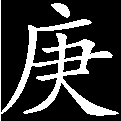
\includegraphics[width=3mm]{../Images/00004}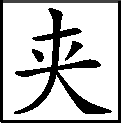
\includegraphics[width=3mm]{../Images/00012}\footnotesize \kaishu 自忙不暇,又加上一``帮''字,可笑可笑。所谓《春秋》笔法。}探春、李纨、迎春、宝钗等也多往那里闲坐,一则观画,二则便于会面。宝钗因见天气凉爽,夜复渐长,{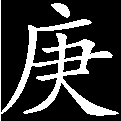
\includegraphics[width=3mm]{../Images/00004}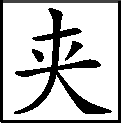
\includegraphics[width=3mm]{../Images/00012}\footnotesize \kaishu ``复''字妙,补出宝钗每年夜长之事,皆《春秋》字法也。}遂至母亲房中商议打点些针线来。日间至贾母处王夫人处省候两次,不免又承色陪坐半时,园中姊妹处也要度时闲话一回,故日间不大得闲,每夜灯下女工必至三更方寝。{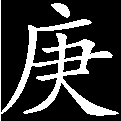
\includegraphics[width=3mm]{../Images/00004}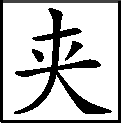
\includegraphics[width=3mm]{../Images/00012}\footnotesize \kaishu {(代)}{[}伏{]}下{(收夕)}{[}后文{]}。◇写针线下``商议''二字,直将寡母训女多少温存活现在纸上。不写阿呆兄,已见阿呆兄终日醉饱优游,怒则吼,喜则跃,家务一概无闻之形景毕露矣。《春秋》笔法。}

黛玉每岁至春分秋分之后,必犯嗽疾;今秋又遇贾母高兴,多游玩了两次,未免过劳了神,近日又复嗽起来,觉得比往常又重,所以总不出门,只在自己房中将养。有时闷了,又盼个姊妹来说些闲话排遣;及至宝钗等来望候他,说不得三五句话又厌烦了。众人都体谅他病中,且素日形体娇弱,禁不得一些委屈,所以他接待不周,礼数粗忽,也都不苛责。

这日宝钗来望他,因说起这病症来。宝钗道:``这里走的几个太医虽都还好,只是你吃他们的药总不见效,不如再请一个高明的人来瞧一瞧,治好了岂不好?每年间闹一春一夏,又不老又不小,成什么?不是个常法。''黛玉道:``不中用。我知道我这样病是不能好的了。且别说病,只论好的日子我是怎么形景,就可知了。''宝钗点头道:``可正是这话。古人说:`食谷者生。'你素日吃的竟不能添养精神气血,也不是好事。''黛玉叹道:``\,`死生有命,富贵在天',也不是人力可强的。今年比往年反觉又重了些似的。''说话之间,已咳嗽了两三次。宝钗道:``昨儿我看你那药方上,人参肉桂觉得太多了。虽说益气补神,也不宜太热。依我说,先以平肝健胃为要,肝火一平,不能克土,胃气无病,饮食就可以养人了。每日早起拿上等燕窝一两,冰糖五钱,用银铫子熬出粥来,若吃惯了,比药还强,最是滋阴补气的。''

黛玉叹道:``你素日待人,固然是极好的,然我最是个多心的人,只当你心里藏奸。从前日你说看杂书不好,又劝我那些好话,竟大感激你。往日竟是我错了,实在误到如今。细细算来,我母亲去世的早,又无姊妹兄弟,我长了今年十五岁,{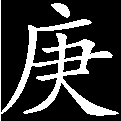
\includegraphics[width=3mm]{../Images/00004}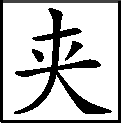
\includegraphics[width=3mm]{../Images/00012}\footnotesize \kaishu 黛玉才十五岁,记清。}竟没一个人像你前日的话教导我。怨不得云丫头说你好,我往日见他赞你,我还不受用,昨儿我亲自经过,才知道了。比如若是你说了那个,我再不轻放过你的;你竟不介意,反劝我那些话,可知我竟自误了。若不是从前日看出来,今日这话,再不对你说。你方才说叫我吃燕窝粥的话,虽然燕窝易得,但只我因身上不好了,每年犯这个病,也没什么要紧的去处。请大夫,熬药,人参肉桂,已经闹了个天翻地覆,这会子我又兴出新文来熬什么燕窝粥,老太太、太太、凤姐姐这三个人便没话说,那些底下的婆子丫头们,未免不嫌我太多事了。你看这里这些人,因见老太太多疼了宝玉和凤丫头两个,他们尚虎视眈眈,背地里言三语四的,何况于我?况我又不是他们这里正经主子,原是无依无靠投奔了来的,他们已经多嫌着我了。如今我还不知进退,何苦叫他们咒我?''

宝钗道:``这样说,我也是和你一样。''黛玉道:``你如何比我?你又有母亲,又有哥哥,这里又有买卖地土,家里又仍旧有房有地。你不过是亲戚的情分,白住了这里,一应大小事情,又不沾他们一文半个,要走就走了。我是一无所有,吃穿用度,一草一纸,皆是和他们家的姑娘一样,那起小人岂有不多嫌的。''宝钗笑道:``将来也不过多费得一副嫁妆罢了,如今也愁不到这里。''{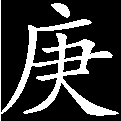
\includegraphics[width=3mm]{../Images/00004}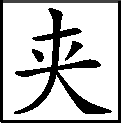
\includegraphics[width=3mm]{../Images/00012}\footnotesize \kaishu 宝钗此一戏,直抵过通部黛玉之戏宝钗矣,又恳切,又真情,又平和,又雅致,又不穿凿,又不牵强。黛玉因识得宝钗后方吐真情,宝钗亦识得黛玉后方肯戏也。此是大关节大章法,非细心看不出。◇细思二人此时好看之极,真是儿女小窗中喁喁也。}黛玉听了,不觉红了脸,笑道:``人家才拿你当个正经人,把心里的烦难告诉你听,你反拿我取笑儿。''宝钗笑道:``虽是取笑儿,却也是真话。你放心,我在这里一日,我与你消遣一日。你有什么委屈烦难,只管告诉我,我能解的,自然替你解一日。我虽有个哥哥,你也是知道的,只有个母亲比你略强些。咱们也算同病相怜。你也是个明白人,何必作`司马牛之叹'?{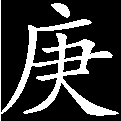
\includegraphics[width=3mm]{../Images/00004}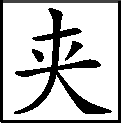
\includegraphics[width=3mm]{../Images/00012}\footnotesize \kaishu 通部众人必从宝钗之评方定,然宝钗亦必从颦儿之评始可,何妙之至!}你才说的也是,多一事不如省一事。我明日家去和妈妈说了,只怕我们家里还有,与你送几两,每日叫丫头们就熬了,又便宜,又不惊师动众的。''黛玉忙笑道:``东西事小,难得你多情如此。''宝钗道:``这有什么放在口里的!只愁我人人跟前失于应候罢了。只怕你烦了,我且去了。''黛玉道:``晚上再来和我说句话儿。''宝钗答应着便去了,不在话下。

这里黛玉喝了两口稀粥,仍歪在床上,不想日未落时天就变了,淅淅沥沥下起雨来。秋霖脉脉,阴晴不定,那天渐渐的黄昏,且阴的沉黑,兼着那雨滴竹梢,更觉凄凉。知宝钗不能来,便在灯下随便拿了一本书,却是《乐府杂稿》,有《秋闺怨》、《别离怨》等词。黛玉不觉心有所感,亦不禁发于章句,遂成《代别离》一首,拟《春江花月夜》之格,乃名其词曰《秋窗风雨夕》。其词曰:

秋花惨淡秋草黄,耿耿秋灯秋夜长。

已觉秋窗秋不尽,那堪风雨助凄凉!

助秋风雨来何速!惊破秋窗秋梦绿。

抱得秋情不忍眠,自向秋屏移泪烛。

泪烛摇摇爇短檠,牵愁照恨动离情。

谁家秋院无风入?何处秋窗无雨声?

罗衾不奈秋风力,残漏声催秋雨急。

连宵脉脉复飕飕,灯前似伴离人泣。

寒烟小院转萧条,疏竹虚窗时滴沥。

不知风雨几时休,已教泪洒窗纱湿。

吟罢搁笔,方要安寝,丫鬟报说:``宝二爷来了。''一语未完,只见宝玉头上戴着大箬笠,身上披着蓑衣。黛玉不觉笑了:``那里来的渔翁!''宝玉忙问:``今儿好些?{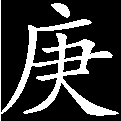
\includegraphics[width=3mm]{../Images/00004}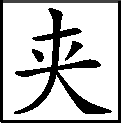
\includegraphics[width=3mm]{../Images/00012}\footnotesize \kaishu 一句。}吃了药没有?{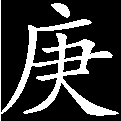
\includegraphics[width=3mm]{../Images/00004}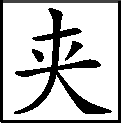
\includegraphics[width=3mm]{../Images/00012}\footnotesize \kaishu 两句。}今儿一日吃了多少饭?''{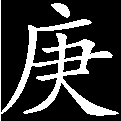
\includegraphics[width=3mm]{../Images/00004}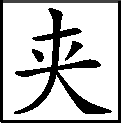
\includegraphics[width=3mm]{../Images/00012}\footnotesize \kaishu 三句。}一面说,一面摘了笠,脱了蓑衣,忙一手举起灯来,一手遮住灯光,向黛玉脸上照了一照,觑着眼细瞧了一瞧,笑道:``今儿气色好了些。''

黛玉看脱了蓑衣,里面只穿半旧红绫短袄,系着绿汗巾子,膝下露出油绿绸撒花裤子,底下是掐金满绣的绵纱袜子,靸着蝴蝶落花鞋。黛玉问道:``上头怕雨,底下这鞋袜子是不怕雨的?也倒干净。''宝玉笑道:``我这一套是全的。有一双棠木屐,才穿了来,脱在廊檐上了。''黛玉又看那蓑衣斗笠不是寻常市卖的,十分细致轻巧,因说道:``是什么草编的?怪道穿上不像那刺猬似的。''宝玉道:``这三样都是北静王送的。他闲了下雨时在家里也是这样。你喜欢这个,我也弄一套来送你。别的都罢了,惟有这斗笠有趣,竟是活的。上头的这顶儿是活的,冬天下雪,戴上帽子,就把竹信子抽了,去下顶子来,只剩了这圈子。下雪时男女都戴得,我送你一顶,冬天下雪戴。''黛玉笑道:``我不要他。戴上那个,成个画儿上画的和戏上扮的渔婆了。''及说了出来,方想起话未忖夺,与方才说宝玉的话相连,后悔不及,羞的脸飞红,便伏在桌上嗽个不住。{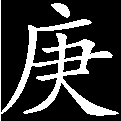
\includegraphics[width=3mm]{../Images/00004}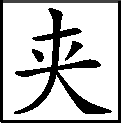
\includegraphics[width=3mm]{../Images/00012}\footnotesize \kaishu 妙极之文。使黛玉自己直说出夫妻来,却又云``画的''``扮的'',本是闲谈,却是暗隐不吉之兆。所谓``画儿中爱宠''是也,谁曰不然?}

宝玉却不留心,{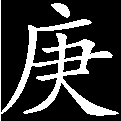
\includegraphics[width=3mm]{../Images/00004}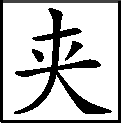
\includegraphics[width=3mm]{../Images/00012}\footnotesize \kaishu 必云``不留心''方好,方是宝玉。若着心则又有何文字?且直是一时时猎色一贼矣。}因见案上有诗,遂拿起来看了一遍,又不禁叫好。黛玉听了,忙起来夺在手内,向灯上烧了。宝玉笑道:``我已背熟了,烧也无碍。''黛玉道:``我也好了些,多谢你一天来几次瞧我,下雨还来。这会子夜深了,我也要歇着,你且请回去,明儿再来。''宝玉听说,回手向怀中掏出一个核桃大小的一个金表来,瞧了一瞧,那针已指到戌末亥初之间,忙又揣了,说道:``原该歇了,又扰的你劳了半日神。''说着,披蓑戴笠出去了,又翻身进来问道:``你想什么吃,告诉我,我明儿一早回老太太,岂不比老婆子们说的明白?''{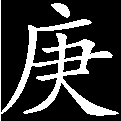
\includegraphics[width=3mm]{../Images/00004}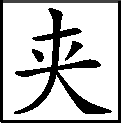
\includegraphics[width=3mm]{../Images/00012}\footnotesize \kaishu 直与后部宝钗之文遥遥针对。◇想彼姊妹房中婆子丫鬟皆有,随便皆可遣使,今宝玉独云``婆子''而不云``丫鬟''者,心内已度定丫鬟之为人,一言一事,无论大小,是方无错谬者也,一何可笑!}黛玉笑道:``等我夜里想着了,明儿早起告诉你。你听雨越发紧了,快去罢。可有人跟着没有?''有两个婆子答应:``有人,外面拿着伞点着灯笼呢。''黛玉笑道:``这个天点灯笼?''宝玉道:``不相干,是明瓦的,不怕雨。''黛玉听了,回手向书架上把个玻璃绣球灯拿了下来,命点一支小蜡来,递与宝玉,道:``这个又比那个亮,正是雨里点的。''宝玉道:``我也有这么一个,怕他们失脚滑倒了打破了,所以没点来。''黛玉道:``跌了灯值钱,跌了人值钱?你又穿不惯木屐子。那灯笼命他们前头点着。这个又轻巧又亮,原是雨里自己拿着的,你自己手里拿着这个,岂不好?明儿再送来。就失了手也有限的,怎么忽然又变出这`剖腹藏珠'的脾气来!''宝玉听说,连忙接了过来,前头两个婆子打着伞提着明瓦灯,后头还有两个小丫鬟打着伞。宝玉便将这个灯递与一个小丫头捧着,宝玉扶着他的肩,一径去了。

就有蘅芜苑的一个婆子,也打着伞提着灯,送了一大包上等燕窝来,还有一包子洁粉梅片雪花洋糖。说:``这比买的强。姑娘说了:姑娘先吃着,完了再送来。''黛玉回说``费心'',命他外头坐了吃茶。婆子笑道:``不吃茶了,我还有事呢。''黛玉笑道:``我也知道你们忙。如今天又凉,夜又长,越发该会个夜局,痛赌两场了。''婆子笑道:``不瞒姑娘说,今年我大沾光儿了。横竖每夜各处有几个上夜的人,误了更也不好,不如会个夜局,又坐了更,又解闷儿。今儿又是我的头家,如今园门关了,就该上场了。''{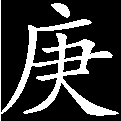
\includegraphics[width=3mm]{../Images/00004}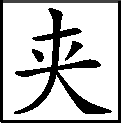
\includegraphics[width=3mm]{../Images/00012}\footnotesize \kaishu 几句闲话,将潭潭大宅夜间所有之事描写一尽。虽偌大一园,且值秋冬之夜,岂不寥落哉?今用老妪数语,更写得每夜深人定之后,各处{[}灯{]}光灿烂、人烟簇集,柳陌{(之)}巷之中,或提灯同酒,或寒月烹茶者,竟仍有络绎人迹不绝,不但不见寥落,且觉更胜于日间繁华矣。此是大宅妙景,不可不写出。又伏下后文,且又衬出后文之冷落。此闲话中写出,正是不写之写也。脂砚斋评。}黛玉听说笑道:``难为你。误了你发财,冒雨送来。''命人给他几百钱打些酒吃,避避雨气。那婆子笑道:``又破费姑娘赏酒吃。''说着,磕了一个头,外面接了钱,打伞去了。

紫鹃收起燕窝,然后移灯下帘,伏侍黛玉睡下。黛玉自在枕上感念宝钗,一时又羡他有母兄;一面又想宝玉虽素习和睦,终有嫌疑。又听见窗外竹梢蕉叶之上,雨声淅沥,清寒透幕,不觉又滴下泪来。直到四更将阑,方渐渐的睡了。暂且无话。要知端的------

{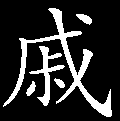
\includegraphics[width=3mm]{../Images/00005}  \kaishu 总评:请看赖大,则知贵家奴婢身份,而本主毫不以为过分,习惯自然,故是有之。见者当自度是否可也。}
